\section{Isoform Quantification}
RSEM, Sailfish and Kallisto are used for transcript-level quantification. Expectation-Maximum (EM) algorithm works by assigning reads to multiple genomic loci and also works without reference genome. Hybrid approaches have been that use the isoform abundance estimates from long-reads to weight the isoform abundance estimated from short-read RNA-Sequencing have been made, however they are not widely adopted\cite{Bayega2018}.

Isoform abundance was determined in two ways, using either a hybrid approach of long and short reads or the normalised full-length long read count as proxy (\cref{fig:isoform_quant_strategy}). The hybrid approach was a modified strategy of typical RNA-Seq quantitive analyses, whereby short reads were aligned to the Iso-Seq defined transcriptome (a merged, comprehensive annotation) rather than the reference genome, thereby improving read alignment to condition-specific transcripts and enabling the detection of novel transcripts. 

Various bioinformatic tools and computational models have been developed to quantify isoform quantification from RNA-Seq data. There are currently two main methods:
\begin{enumerate}
	\item Inclusion level, calculated for a regulated exon by aligning reads either to candidate alternative exons and its junctions (inclusion reads), or to flanking exons and subsequently skipping the candidate alternative exon (skipping/exclusion reads) (Chen et al. 2012)
	\item Percent-Spliced-In (PSI\nomenclature{PSI}{Percent-Spliced In}), calculated by proportion of isoforms that include the exon (Venables et al. 2008)(Katz et al. 2010). If the PSI value is calculated for a particular splicing event, it can be considered equivalent to the inclusion level. 
\end{enumerate}
Isoform quantification can either be expressed as a global measure of expression, which provides a global gene expression ranking in one sample (measured by RPKM: Reads of a transcript sequence per Millions mapped read\nomenclature{RPKM}{Reads of a transcript sequence per Millions}), or as a relative measure of expression, which is normalized per gene locus and comparable across conditions (measured by inclusion level or PSI value). 

Isoform abundance calculated by aligning short-reads to transcriptome is preferential to alignment with reference annotation library (RefSeq/GENCODE) in narrowing down the isoforms expressed and thus subsequently enabling more reliable abundance quantification. Reference annotation library is constructed on all data from the same species, and inclusion of annotated but not truly expressed isoforms can increase variability of abundance estimates. Finally, if the reference library is incomplete, then truly expressed isoforms would be completely missed and RNA-Seq reads would be incorrectly assigned to annotated isoform (\cite{Au2013})

\begin{figure}[htp]
	\begin{center}
		\includegraphics[page=8,trim={2cm 19cm 0 1cm},clip, scale = 0.8]{Figures/ProjectDevelopment_Figures.pdf}
	\end{center}
	\captionsetup{width=0.95\textwidth}
	\caption[Strategies for isoform quantification]%
	{\textbf{Strategies for isoform quantification using long and short reads}: A schematic diagram of three strategies adopted for determining isoform abundance, using either short RNA-Seq reads aligned to the reference genome or the Iso-Seq defined transcriptome (hybrid approach), or the normalised full-length read count directly from long reads}
	\label{fig:isoform_quant_strategy}
\end{figure}


\boldheader{Removal of ISM and merging of FSM}
Following \textit{SQANTI} annotations, there were many examples where multiple ISM and several FSM transcripts were annotated to the same known isoform (exemplified in \cref{fig:redudant_sncatranscripts}). This is likely due to varying extent of 5'degradation and truncation - small degree of degradation or truncation would result in differing 5' and 3' ends respectively while preserving the internal exonic structure and thereby generating several FSM; conversely, a large degree of degradation or truncation would generate smaller partial isoforms that also have matching, albeit smaller overlap, exonic structure. To ease downstream quantitative analyses, ISM and shorter FSM were assumed as partial products of the longest detected FSM transcript, and the associated counts were aggregated (as shown in \cref{fig:ism_collapse}). However, there is a caveat that significantly shorter ISM transcripts could in theory be mapped to multiple isoforms.  

\begin{figure}[htp]
	\begin{center}
		\includegraphics[page=10,trim={0cm 0cm 0 0cm},clip, scale = 0.7]{Figures/ProjectDevelopment_Figures.pdf}
	\end{center}
	\captionsetup{width=0.95\textwidth}
	\caption[Redundant ISM and FSM associated with same known isoform]%
	{\textbf{Redundant ISM and FSM associated with known transcript of \textit{Snca}}: \textbf{a)} Visualising transcripts using \textit{Swan}, shown are \textbf{b)} transcripts detected after \textit{SQANTI} annotation of the mouse transcriptome using the targeted approach. An example of detecting multiple redundant transcripts annotated to the same isoform, all the transcripts depicted were annotated to ENMUST0000014268.4 which typically differed at the 5' and 3' end.}
	\label{fig:redudant_sncatranscripts}
\end{figure}

\begin{figure}[htp]
	\centering
	\includegraphics[page=9,trim={0cm 12cm 0cm 0cm},clip,scale = 0.8]{Figures/ProjectDevelopment_Figures.pdf}
	\captionsetup{width=0.95\textwidth,singlelinecheck=off}
	\caption[Merging of ISM and FSM]%
	{\textbf{Merging of ISM and FSM associated with the same known isoform}. All illustration of handling with multiple ISM and FSM associated with the same known transcript. In this example, 6 isoforms were detected for "Gene 1", however, only 4 known isoforms were identified (denoted as ENMUST1-4). For ease of annotation and quantification, ISM and shorter FSM were assumed partial products of the longer FSM. Consequently, in the case where: 
		\begin{itemize}
			\item both ISM (PB.1.2) and FSM (PB.1.1) are annotated to the same transcript (shaded green), the FSM takes precedence as the associated transcript and counts from respective ISM are aggregated 
			\item there is one ISM (PB.1.3) but no corresponding FSM for the associated transcript (shaded blue), the ISM is retained
			\item there are multiple ISM (PB.1.4, PB.1.5) annotated to the same transcript (shaded orange), the longest ISMs (PB.1.5) takes precedence and counts from respective ISM are similarly aggregated 
			\item there are multiple FSM (PB.1.6, PB.1.7) annotated to the same transcript (shaded purple), the longest FSM (PB.1.7) takes precedence and counts are similarly aggregated
			\\
		\end{itemize} 
		PB - PacBio. FSM - Full Splice Match, ISM - Incomplete Splice Match, FL - Full-length read counts.  
	}
	\label{fig:ism_collapse}
\end{figure}

\clearpage
\boldheader{RNA-Seq Alignment to Iso-Seq defined transcriptome}
For the hybrid approach of aligning short reads to Iso-Seq defined transcriptome from the targeted approach, several factors were optimised including the library size and the Iso-Seq annotation (\cref{tab:rnaseq_alignment_targeted}) to align RNA-Seq reads to targeted transcriptome dataset using \textit{Kallisto}. 

\begin{table}[h]
	\centering
	\caption[RNA-Seq Alignment strategy to Iso-Seq defined targeted transcriptome]%
	{\textbf{RNA-Seq Alignment strategy to Iso-Seq defined targeted transcriptome}. Tabulated is trialled methods of aligning short reasd to Iso-Seq defined transcriptome, with alterations either of the sequencing library (such as the pool of the sequencing reads for alignment) and the choice of Iso-Seq isoform for alignment}
	\label{tab:rnaseq_alignment_targeted}
	\begin{threeparttable}
		\begin{tabular}{@{}cll@{}}
			\toprule
			Method & Sequencing Library                       & Annotation                            \\ \midrule
			1      & Targeted Transcriptome (All Reads)\tnote{a}       & No Isoform collapse\tnote{c}                   \\
			2      & Targeted Transcriptome (All Reads)\tnote{a}       & Isoform collapse to longest FSM\tnote{d}       \\
			3      & Targeted Transcriptome (All Reads)\tnote{a}       & Isoform collapse to most abundant FSM\tnote{e} \\
			4      & Targeted Transcriptome (On-Target Reads)\tnote{b} & Isoform collapse to longest FSM\tnote{d}       \\
			5      & Targeted Transcriptome (On-Target Reads)\tnote{b} & Isoform collapse to most abundant FSM\tnote{e} \\
			6 & \begin{tabular}[c]{@{}l@{}}Whole Transcriptome \& \\ Targeted Transcriptome (On Target Reads)\end{tabular} & Isoform collapse to longest FSM \\ \bottomrule
		\end{tabular}
		\begin{tablenotes}
			\footnotesize
			\item[a] Sequencing reads from on-target and off-target genes
			\item[b] Sequencing reads aligned only to on-target genes
			\item[c] Transcriptome annotation following \textit{SQANTI} with no removal of redundant ISM and FSM
			\item[d] Transcriptome annotation following \textit{SQANTI} with collapse of redundant ISM to respective longest FSM of same transcript and aggregated counts
			\item[e] Transcriptome annotation following \textit{SQANTI} with collapse of redundant ISM to respective most abundant FSM of same transcript and aggregated counts 
		\end{tablenotes}
	\end{threeparttable}
\end{table}

However, independent of the scaffold or library size, \textit{Kallisto} appeared to mis-assign short reads to novel isoforms. This is exemplified with \textit{Clu} (\cref{fig:Clu_TargetedRNAseqAlignment}) and \textit{Bin1} (\cref{fig:Bin1_TargetedRNAseqAlignment}).   Using total Iso-Seq FL reads from targeted transcriptome as proxy of transcript expression, the known and longer isoforms associated with both \textit{Clu} (\cref{fig:Clu_TargetedRNAseqAlignment}\textbf{a}) and \textit{Bin1}(\cref{fig:Bin1_TargetedRNAseqAlignment}\textbf{a}) were most abundant whereas the novel isoforms were only lowly detected. Conversely, alignment of RNA-Seq reads to targeted transcriptome often ascribed the novel isoforms as the dominant isoform(s), particularly when further collapsing targeted transcriptome to longest or most abundantly expressed isoforms or limiting the scaffold to only on-target reads (Methods 2 - 5 from \cref{tab:rnaseq_alignment_targeted}). Nonetheless, while using all the reads from the targeted transcriptome with redundant ISM and FSM is more likely to ascribe the known isoform as the dominant isoform, mis-asignment can still occur with the shorter, redundant ISM annotated as most abundantly expressed rather than the longer, complete FSM (\cref{fig:Clu_TargetedRNAseqAlignment}\textbf{a, b, d}).

Visualisations of the dominant known isoform ascribed by Iso-Seq FL read counts and the dominant novel isoform ascribed by RNA-Seq alignment from \textit{Clu} and \textit{Bin1} show that both isoforms are structurally very similar, with almost identical internal exonic structure bar one or two exons with differing splice junctions. There was no difference in RNA-Seq coverage from \textit{Kallisto} alignment to targeted transcriptome across all the methods \cref{tab:rnaseq_alignment_targeted}), suggesting that the issue is the probabilistic assignment of reads to isoforms (Expectation-Maximum algorithm) rather than the alignment. It appears that in cases where the known and novel isoforms are similar in transcript structure, and consequently there are only a few short reads that can be unambiguously assigned, \textit{Kallisto} fails to quantify at an isoform level. Given that significantly more novel isoforms are identified using the targeted approach than the whole transcriptome approach, this is more likely to be evident in the former.   


\newgeometry{left=0.5cm,top=1cm,right=0.5cm}
\begin{landscape}
	\begin{figure}[htp]
		\centering
		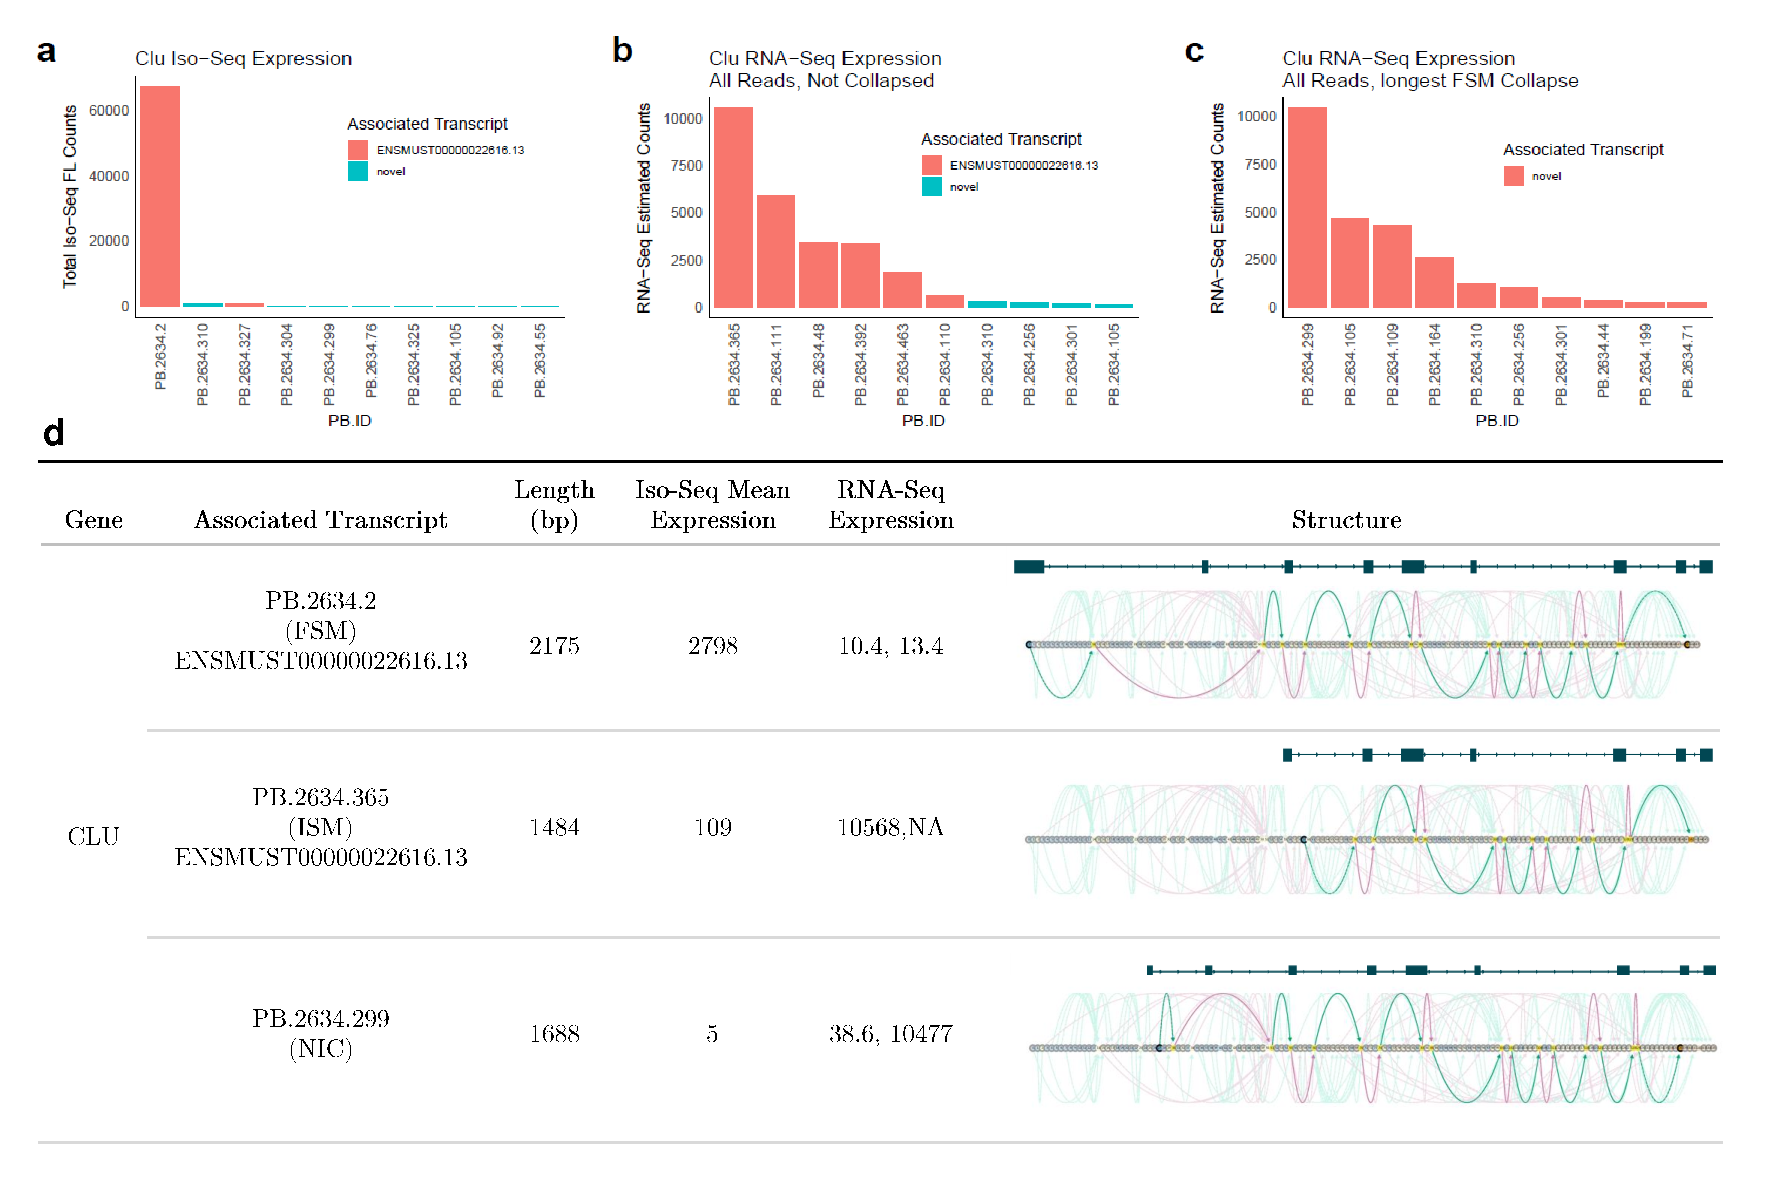
\includegraphics[page=1,trim={0cm 1cm 0cm 0cm},clip,scale = 0.8]{Figures/ProjectDevelopment_Figures_Landscape.pdf}
		\captionsetup{width=1.2\textwidth,singlelinecheck=off}
		\caption[RNA-Seq mis assignment of dominant isoform associated with \textit{Clu}]%
		{\textbf{RNA-Seq mis assigns \textit{Clu}'s novel isoform as most abundantly expressed}. Shown are the top 10 most abundantly expressed \textit{Clu} transcripts based on \textbf{a)} Iso-Seq full-length read counts from targeted transcriptome, \textbf{b)} RNA-Seq reads aligned to all reads in targeted transcriptome, with no further collapse of redundant FSM and ISM transcripts (Method 1 in \cref{tab:rnaseq_alignment_targeted}) and \textbf{c)} RNA-Seq reads aligned to all reads in targeted transcriptome with isoforms further collapsed to longest FSM (Method 2 in \cref{tab:rnaseq_alignment_targeted}). Of note, all other methods (3 - 6) generated a similar plot to figure c. \textbf{d)} Swan visualisations of most abundantly expressed isoforms according to respective methods. Iso-Seq mean expression refer to average full length read counts from targeted transcriptome. RNA-Seq mean expression refer to estimated counts from \textit{Kallisto} in Figures b and c. 
		}
		\label{fig:Clu_TargetedRNAseqAlignment}
	\end{figure}
	
	
	\begin{figure}[htp]
		\centering
		\includegraphics[page=2,trim={0cm 0cm 0cm 0cm},clip,scale = 0.8]{Figures/ProjectDevelopment_Figures_Landscape.pdf}
		\captionsetup{width=1.2\textwidth,singlelinecheck=off}
		\caption[RNA-Seq mis-assignment of dominant isoform associated with \textit{Bin1}]%
		{\textbf{RNA-Seq mis-assigns \textit{Bin1}'s novel isoform as most abundantly expressed}. Shown are the top 10 most abundantly expressed \textit{Bin1} transcripts based on \textbf{a)} Iso-Seq full-length read counts from targeted transcriptome, \textbf{b)} RNA-Seq reads aligned to all reads in targeted transcriptome, with no further collapse of redundant FSM and ISM transcripts (Method 1 in \cref{tab:rnaseq_alignment_targeted}) and \textbf{c)} RNA-Seq reads aligned to all reads in targeted transcriptome with isoforms further collapsed to longest FSM (Method 2 in \cref{tab:rnaseq_alignment_targeted}). Of note, all other methods (3 - 6) generated a similar plot to figure c. \textbf{d)} Swan visualisations of most abundantly expressed isoforms according to respective methods. Iso-Seq mean expression refer to average full length read counts from targeted transcriptome. RNA-Seq mean expression refer to estimated counts from \textit{Kallisto} in Figures b and c. 
		}
		\label{fig:Bin1_TargetedRNAseqAlignment}
	\end{figure}
\end{landscape}
\restoregeometry

\subsubsection{Iso-Seq isoform expression}
To control for sequencing bias in library depth, full-length (FL) read count for each isoform is normalized to transcripts per million (TPM \nomenclature{TPM}{Transcripts per Million})), which is calculated as: 

\begin{align*}
	FL\;\:TPM (x_{sample},y_{sample})=\frac{Raw\;\:FL\;\:count (x_{isoform},y_{sample})}{Total\;\:FL\;\:count (y_{sample})} *10^6
\end{align*}

With a cut-off lower than 0.5 TPM, a 0.5 - 10 TPM refers to low expression, a 11- 1000 refers to medium expression, and > 1000 TPM high expression [literature ref]. 

TPM is the most effective within-sample normalisation method to relatively quantify gene expression in a sample \cite{Abrams2019}. Other methods include RPKM (reads per kilobase of transcripts per million mapped reads), FPKM (fragments per kilobase of exon model per million mapped reads), which uses gene length to control for fragmentation in RNA-Seq protocol ("effective length normalisation") - however, this is not necessary in Iso-Seq.  

Between-sample normalisation methods to relatively quantify expression of the same gene in different samples, remove technical variations due to presence of few highly expressed genes that make up a significant proportion of total reads, and due to different number of reads in each sample. 